\cotefile{156-7}
\scanpage{2}
\mspage{1}
\margin{\tikz[baseline=(h.base)]{\node[inner sep=2pt] (h) {\unsure{GF|CF} VII}; \draw (h.north west)--(h.south west)--(h.south east);}}
\begin{center}Analysis Situs (troisième mouture)\end{center}
% slanted
\margin{Cf surtout p. 23 50-58, 59 \tikz[baseline=(q.base)]{\node[inner sep=2pt] (q) {110-113}; \draw[->] (q.north)..controls (q.north east) and (q.north east)..(q.east)..controls (q.south east) and (q.south east)..(q.south)..controls (q.south west) and (q.south west)..(q.west)..controls (q.north west) and (q.north west)..(q.north);}}

\uline{23 juin}

Je récapitule les données et axiomes d'une ``algèbre des figures'', ou ``\uline{atelier}''. \margin{--}Il s'agit pour l'instant d'axiomes purement ``algébriques'' dominant le formalisme algébrique des figures, à l'exclusion pour le moment des propriétés topologiques (densité, connexité, acyclicité) ou \inserted{\uline{proprement}} géométriques (régularité topologique, boules et sphères topologiques d'une algèbre de figures), voire les ``propriété combinatoires fines'', autour de la notion de simplexe.

Parmi les axiomes, je distingue les axiomes ``sine qua non'' At~1 à At~7, qui me paraissent les plus essentielles pour fonder le sens géométrico-topologique du formalisme envisagé. Les autres axiomes seront considérés comme plus ou moins ``facultatifs'' au niveau du formalisme algébrique. Ils pourront sans \unsure{doute} un rôle crucial, dès qu'il s'agira d'un travail sur piéces dans le

\scanpage{3}
\mspage{2}
contexte d'un atelier définissant une ``contrée''.

Le travail précédent a permis de dégager le point de vue le plus commode pour le formalisme algébrique. La notion fondamentale me semble bien celle de \uline{figure}, et non pas celle de ``figure élémentaire'' ou ``multistrate'', voire celle de ``lieu'' (voire, la notion de ``lieu ponctuel'' ou ``point'', dont il n'a pas encore été question\ldots). Une des raisons en est la simplicité du formalisme algébrique,
% slanted
\margin{L'autre raison, c'est que, dans le cas d'une ``application $f$'' d'une ``région'' dans une autre, l'image inverse d'une ``figure'' (\unsure{quand|quant} \unsure{on} peut donner un sens \unsure{géométrique} \unsure{à} \unsure{ce} \unsure{mot|terme}) \deleted{\unsure{sera}} tend à ne \unsure{pas} être \unsure{encore} une figure, mais l'image réciproque d'une multistr. est une multistr.}%
 où il est agréable de pouvoir manipuler les lieux et multistrates comme étant des figures particulières. Quand une figure \inserted{$F$} est interprétée \inserted{(par l'ens de ses ``strates'')} comme partie de l'ens $\unsure{M|\mathcal M}$ \inserted{(ordonné par $\leq$)} des multistrates, nous allons écrire $\widetilde F$ (et non $F$) pour cette partie. Quand elle est interprétée comme une figure \inserted{ensembliste} dans $M$, nous l'écrivons $\mathrm{Mulomb}(F)$ (``grande multiombre''), son support est $\mathrm{Omb}(F)$ (la ``grande ombre'' de $F$) -- cette dernière, contrairement à $\widetilde F$ et à $\mathrm{Mulomb}(F)$, ne permet pratiquement jamais de réconstituer $F$, \deleted{\unsure{le|il}} mais moralement, son ``support'' seulement

\scanpage{4}
\mspage{3}
(et je suis resté muet sur ce support dans la mouture précédente \unsure{GF|CF} $\underline{\overline{\mathrm{VI}}}$). Quand on interprète $F$ comme figure ensembliste dans l'ens. des lieux $\unsure{L|\mathcal L}$ \deleted{\unsure{ou|de}} (pratiquement cela signifie qu'on a un atelier ensembliste), on l'écrira $\mathrm{mulomb}(F)$ (petite multiombre), son support sera $\mathrm{omb}(F)$.

\uline{Données} \uline{pre\deleted{\unsure{l|li|pré}}mières} :
\[
\left\{\begin{aligned}
&\unsure{\mathscr F|\mathcal F} &&\text{ensemble de figures}\\
&\leq &&\text{rellation d'\uline{inclusion} de figures}\\
& &&F\leq G\ \overset{\text{\unsure{déf|def}}}{\Longleftrightarrow}\ F\ \text{sous figure de }G\\
&\ll &&\text{relation de raffinement}\\
& && F\ll G\ \overset{\text{def}}{\Longleftrightarrow}\ F\ \text{raffine }G
\end{aligned}\right.
\]
avec
\[
F\leq G\ \Longrightarrow\ F\ll G\tag*{\makebox[0pt][r]{\makebox[\displaywidth][l]{\uline{At} 0}}}
\]
% slanted
\margin{NB. Ce sera aussi contenu dans \uline{At}~4 plus bas}
-- axiome si évident que je ne l'avais pas inclus dans les axiomes numérotés.

\diagram{\(\begin{array}{@{}clp{.53\linewidth}@{}}
\text{\textcircled{\scriptsize a}} & F\vee G\ \text{ou }F\cup G &
\uline{figure} ``\uline{engendrée}'' ou ``\uline{réunion}'' ou ``\uline{somme}'' : c'est le sup au sens de $\leq$ (quand il existe\unsure{\}|)} -- auquel cas c'est aussi un sup pour $\ll$\\
\end{array}\)}
\margin{\deleted{Question}\inserted{NB.} : Si $(F,G)$ ont un sup pour $\ll$ (c'est tjrs le cas dans le cas ensembliste $\mathrm{Fig}(L)$), ce n'est pas néc. un sup pour $\leq$}
\margin{\uline{NB} $\widetilde{F\cap G}=\widetilde F\cap\widetilde G$}
\diagram{\(\begin{array}{@{}clp{.53\linewidth}@{}}
\text{\textcircled{\scriptsize b}} & \begin{aligned}&F\wedge G\ \text{ou } F\cap G\\&\quad(=\mathrm{Inf}^{\leq}(F,c))\end{aligned}
& figure \uline{intersection}\inserted{ou Inf pour $\leq$} -- existe toujours ($\overline{\mathrm m}$ pour \unsure{familles|famille} infinie (non vide)) ; quand en $=$ temps $F\vee\unsure{C|G}$ existe, alors c'est aussi le Inf pour $\ll$.\\
\end{array}\)}
\margin{\uline{NB} Existe dans le cas ensembliste $\mathrm{Fig}(L)$ et dans le cas \unsure{mechisé|méchisé}}
\diagram{\(\begin{array}{@{}clp{.53\linewidth}@{}}
\text{\textcircled{\scriptsize\unsure{c}}} & F\mathbin{\ldotp}G\quad (=\mathrm{Inf}^{\ll}(F,c)) &
figure ``\uline{intersection} \uline{fine}'' (quand elle existe) : Inf pour $\ll$.\\
&\deleted{\unsure{CG|G}}&\\
\text{\textcircled{\scriptsize\unsure{d}}} & \varnothing_{\mathscr F} &
figure vide : plus petit élément de $\mathscr F$ (pour $\leq$ \uline{et} pour $\ll$)\\
\end{array}\)}

\scanpage{5}
\mspage{\deleted{\unsure{3}}4}
\textcircled{\scriptsize\unsure{e}} $\unsure{M|\mathcal M}={}$ ensemble des \unsure{``}\uline{figures} $\subset\unsure{\mathscr F|\mathcal F}$ \uline{élémentaires}'' ou \uline{multistrates}

% Upper left margin; ruled connection to item e.
\reversemarginpar
\margin{\tikz[x=.6em,y=.6em]{\draw (0,1.7)--(0,2.85) .. controls (0,3.06) and (.19,3.12) .. (.50,3.12)--(2.55,3.18) .. controls (2.80,3.19) and (2.85,3.62) .. (2.88,3.9); \draw (0,1.7)--(1.20,1.72)--(2.88,1.53)--(3.02,0);}\enspace\uline{strates} d'une figure : les $X\in M$ tels que $X\leq F$\\ \uline{déployement} de $F$ : ens. de ses \uline{strates}\\ $\widetilde F=\{X\in M\mid X\leq F\}$\\ On écrit $X\triangleleft F$ ($X$ \uline{incident} à $F$) pour $X\in M$ et $X\leq F$}
\normalmarginpar
% Upper right column, aligned with item e.
\margin{formé des objets de $(\mathscr F,\leq)$ strictement irréductibles. Muni des relations $\underset{M}{\leq}$, $\underset{M}{\ll}$ induites par \deleted{\unsure{$\mathscr F$}} $\leq$ et $\ll$ dans $\mathscr F$}

\textcircled{\scriptsize\unsure{f}} $\unsure{L|\mathcal L}\subset M$, ens. des \deleted{\uline{\unsure{éléments}}} \inserted{``lieux''} \deleted{\unsure{minimaux}}
\inserted{\tikz[x=.7em,y=.7em]{\draw (0,1.27)--(1.72,1.22) .. controls (2.06,1.22) and (2.42,1.02) .. (2.75,.85)--(4.67,.04)..controls(4.87,.17)and(5.17,.06)..(5.43,.08); \draw (2.57,.93)..controls(2.80,.54)and(4.13,.21)..(4.67,.04);}\enspace éléments minimaux de $\mathscr F\setminus\{\varnothing_{\mathscr F}\}$ pour $\ll$}

\uline{Axiomes}

I) Axiomes ``sine qua non''. Les premiers trois \inserted{At~1 - At~3} ne concernent que $(\mathscr F,\leq)$, les quatre suivants At~4 - At~7 \deleted{\unsure{At 1|At 4}} \deleted{\unsure{4|et}} les relations entre $\leq$ et $\ll$

% Slanted left margin beside At 1.
\reversemarginpar
\margin{Axiomes des \uline{sommes majorées de figures}}
\uline{At 1}\quad $\mathscr F\neq\varnothing$ et stable par $\underset{I}{\mathrm{Sup}}$ majorés ($I$ quelconque)

% Slanted left margin beside At 2.
\margin{Axiome des strates équivaut à :\\ Si $F,\unsure{C|G}\in\mathscr F$, alors\\ $F\leq G\Longleftrightarrow\forall X\in\widetilde F,\ \exists Y\in\widetilde G$ avec $X\leq Y$\\ Critère \uline{d'inclusion de figures par strates}}
\uline{At 2}\quad Toute figure \deleted{\unsure{d}}est le sup de ses strates :
\[
 F=\underset{X\in\widetilde F}{\mathrm{Sup}}\,X\qquad\text{où}\qquad
 \widetilde F=\{X\in M\mid X\leq F\}
\]

\uline{Scholie}\qquad \uline{At}~1 et \uline{At}~2 signifient que $\mathscr F$ s'interprète, via $F\mathrel{\tikz[baseline=-.45ex,x=.7em,y=.45em]{\draw (0,-.44)--(0,.44) (0,0)--(1.2,0) (1.2,-.44)--(1.2,.44);}}\widetilde F$, comme une \unsure{parties|partie} $\widetilde{\mathscr F}$ de $\mathscr F(M)$, $M$ ens ordonné (pour $\leq$), avec les conditions :

a) les $\unsure{\Phi|\varphi}\in\widetilde{\mathscr F}$ sont fermés

b) Si $\Phi\in\widetilde{\mathscr F}$, toute partie fermée de $\Phi$ est $\in\widetilde{\mathscr F}$

c) $\deleted{\widetilde{\mathscr F}\neq\varnothing\quad(\Longleftrightarrow\varnothing\in\widetilde{\mathscr F})}$ \deleted{\unsure{(et}} $\displaystyle\bigcup_{\Phi\unsure{+|\in}\widetilde{\mathscr F}}\Phi=M$, et $\widetilde{\mathscr F}\neq\varnothing$
% Slanted left margin beside clause c.
\margin{$\widetilde{\mathscr F}\neq\varnothing$ automatique si $M\neq\varnothing$\\ et dans tous les cas, \unsure{équivaut}\enspace\tikz[baseline=-.3ex,x=.65em,y=.65em]{\draw[->] (0,0) .. controls (.65,.05) and (1.8,.7) .. (2.9,1.7);}\\ à $\varnothing\in\widetilde{\mathscr F}$}

ou, indépendamment d'une relation d'ordre sur $M$, un ens de parties satisfaisant
\diagram{\begin{tikzcd}[ampersand replacement=\&,column sep=0pt,row sep=2ex]
{} \& |[align=left,text width=.83\linewidth]| \text{b$'$)}\quad \forall x\in M,\ \text{l'ens } \widetilde{\mathscr F}^{x}=\{\deleted{\unsure{F}}\Phi\in\overline{\mathscr F}\mid x\in\Phi\}\ \text{a un} \\
{} \& |[align=left,text width=.83\linewidth]| \text{plus petit élément }\deleted{F}\ \text{(noté }\widetilde X\text{)}\\
{}\arrow[uu,bend left=35] \& |[align=left,text width=.83\linewidth]| \text{a$'$)}\quad\deleted{\unsure{\forall|F}}\ \text{Dans }(\widetilde{\mathscr F},\subset),\ \text{\unsure{toutes|toute} famille}\\
{} \& |[align=left,text width=.83\linewidth]| \text{majorée a un Sup, \uline{et} }\widetilde{\mathscr F}\neq\varnothing\\
{} \& |[align=left,text width=.83\linewidth]| (\Longleftrightarrow\varnothing\in\widetilde{\mathscr F})
\end{tikzcd}}

\normalmarginpar
Relation
\[
\begin{aligned}
F\mathrel{\tikz[baseline=-.4ex,x=.65em,y=.65em]{\draw (0,1.1)--(1,.5)--(0,-.1) (1,1.1)--(0,.5)--(1,-.1);}}G
&\overset{\text{\unsure{dfn|defn}}}{\Longleftrightarrow}
 F\vee C\ \text{existe i.e. }\{F,G\}\ \text{majoré dans }(\mathscr F,\leq)\\
&\text{\uline{figures} \uline{compatibles}}
\end{aligned}
\]
Cette relation induit $X\mathrel{\tikz[baseline=-.4ex,x=.65em,y=.65em]{\draw (0,1.1)--(1,.5)--(0,-.1) (1,1.1)--(0,.5)--(1,-.1);}}Y$ dans $M$. Dans le cas où les figures sont de t.f., alors $(\mathscr F,\leq)$ \deleted{\unsure{est}} \inserted{\tikz[baseline=(t.base),x=.65em,y=.65em]{\node[inner sep=0,anchor=west] (t) at (.6,1) {avec At~1, At~2, At~3};\draw[->] (t.south east)--++(0,-.25)--(.8,.3) .. controls (.2,.3) and (.3,0) .. (0,0);}} se reconstitue par
\[
(M,\leq,\mathrel{\tikz[baseline=-.4ex,x=.65em,y=.65em]{\draw (0,1.1)--(1,.5)--(0,-.1) (1,1.1)--(0,.5)--(1,-.1);}}),\quad\text{où }\mathrel{\tikz[baseline=-.4ex,x=.65em,y=.65em]{\draw (0,1.1)--(1,.5)--(0,-.1) (1,1.1)--(0,.5)--(1,-.1);}}\text{ satisfait}
\]
\[
\left\{\begin{aligned}
&X\ \mathrel{\tikz[baseline=-.4ex,x=.65em,y=.65em]{\draw (0,1.1)--(1,.5)--(0,-.1) (1,1.1)--(0,.5)--(1,-.1);}}\ \text{réflexive symétrique}\\
&X\mathrel{\tikz[baseline=-.4ex,x=.65em,y=.65em]{\draw (0,1.1)--(1,.5)--(0,-.1) (1,1.1)--(0,.5)--(1,-.1);}}Y,\ X'\leq X,\ Y'\leq Y\ \Longrightarrow\ X'\mathrel{\tikz[baseline=-.4ex,x=.65em,y=.65em]{\draw (0,1.1)--(1,.5)--(0,-.1) (1,1.1)--(0,.5)--(1,-.1);}}Y'
\end{aligned}\right.
\]

\scanpage{6}
\mspage{5}
Donc la donnée de $(\unsure{\mathscr F|\mathcal F},\leq)$ avec figures de t.f. équivaut : $(\unsure{M|\mathcal M},\leq\deleted{\unsure{X\leq}\mathrel{\tikz[baseline=-.4ex,x=.65em,y=.65em]{\draw (0,1.1)--(1,.5)--(0,-.1) (1,1.1)--(0,.5)--(1,-.1);}}}\text{ (ordre)},\ \mathrel{\tikz[baseline=-.4ex,x=.65em,y=.65em]{\draw (0,1.1)--(1,.5)--(0,-.1) (1,1.1)--(0,.5)--(1,-.1);}}\text{ (relation réflexive sym)}),$ satisfaisant

a) \deleted{$\unsure{\forall x\in M}$, \inserted{posant} $\widetilde X=\{y\in M\mid y\leq x\}$ \unsure{être}} Toute partie fermée majorée $\unsure{\Phi|\varphi}$ de $M$ est de type fini (i.e. \unsure{\deleted{$\exists$}|$\exists$}réunion finie d'ens. $\widetilde X=M_{\leq x}$)
% Left margin, horizontal.
\reversemarginpar
\margin{On aura alors $\widetilde{\mathscr F}={}$ ens des parties fermées de $M$, de type fini, formées \unsure{de|des} éléments deux à deux compatibles (pour $\mathrel{\tikz[baseline=-.4ex,x=.65em,y=.65em]{\draw (0,1.1)--(1,.5)--(0,-.1) (1,1.1)--(0,.5)--(1,-.1);}}$)}

\[
\text{b)}\quad X\mathrel{\tikz[baseline=-.4ex,x=.65em,y=.65em]{\draw (0,1.1)--(1,.5)--(0,-.1) (1,1.1)--(0,.5)--(1,-.1);}}Y,\ X'\leq X,\ Y'\leq Y\ \Longrightarrow\ X'\mathrel{\tikz[baseline=-.4ex,x=.65em,y=.65em]{\draw (0,1.1)--(1,.5)--(0,-.1) (1,1.1)--(0,.5)--(1,-.1);}}Y'.
\]

% Slanted left margin
\margin{Critère de \uline{compatibilité} \uline{par strates}}
\uline{At 3}\quad Soient $F,G\in\mathscr F$ tels que $\forall\deleted{\unsure{x}}X\in\widetilde F,\ Y\in\widetilde{\unsure{C|G}}$, on ait $X\mathrel{\tikz[baseline=-.4ex,x=.65em,y=.65em]{\draw (0,1.1)--(1,.5)--(0,-.1) (1,1.1)--(0,.5)--(1,-.1);}}Y$, alors $F\mathrel{\tikz[baseline=-.4ex,x=.65em,y=.65em]{\draw (0,1.1)--(1,.5)--(0,-.1) (1,1.1)--(0,.5)--(1,-.1);}}G$ (i.e. $F\vee G$ existe)

\deleted{At} Les axiomes suivants concernent les relations entre $\leq$ et $\ll$. \unsure{1}

% Slanted left margin
\margin{Critère de \uline{raffinement} \uline{par strates}\\ [\uline{Corollaire} $F\leq G\Longrightarrow F\ll G$]}
\uline{At}~4\quad $\forall F,\unsure{c|G}\in\mathscr F,$
\[
F\ll G\ \Longleftrightarrow\ \forall X\in\widetilde F,\exists Y\in\widetilde G,\ \text{t.q. }X\ll Y
\]
\inserted{Ramène la connaissance de $\ll$ dans $\mathscr F$ à celle de $\underset{M}{\ll}$}

% Slanted left margin
\margin{\tikz[x=.6em,y=.6em]{\draw (0,0)..controls(.2,.55)and(.65,.95)..(.95,1.15);\draw (1.02,1.22)--(1.14,1.3);}\enspace Axiome de la plus petite strate, ou du \uline{raffinement interne}\quad\tikz[x=.6em,y=.6em]{\draw[->] (0,0) .. controls (1.4,.35) and (2.1,.65) .. (2.85,.7);}}
\uline{At} \deleted{\unsure{5}}6\quad $\unsure{\deleted{\forall}|\forall} X,F\in\mathscr F,\ X\triangleleft F$ (i.e $X\in\widetilde F$), soit $F^{X}=\{Y\in\widetilde F\mid X\deleted{\unsure{\leq}}\ll Y\}$, Alors $F^{x}$ a un plus petit élément.

Notation
\[
\begin{aligned}
X\overset{\circ}{\ll}Y&\ \overset{\text{\unsure{dfn|defn}}}{\Longleftrightarrow}\ X\text{ est plus petit élément de }\widetilde Y^{x}\\
&\text{i.e.}\quad X\ll Y,\quad\text{et } X\ll Y'\triangleleft Y\Longrightarrow Y'=Y\\
(\text{ou } X\in\mathrm{Omb}(Y)^{\circ}) &\qquad X\ \text{\uline{raffinement interne} de }Y
\end{aligned}
\]

% Slanted left margin
\margin{\tikz[x=.6em,y=.6em]{\draw (0,0)..controls(1,.95)and(2.2,1.65)..(3.05,1.9)..controls(3.32,1.99)and(3.55,1.81)..(3.75,1.62); \draw (1.18,2.12)..controls(1.2,1.81)and(1.43,1.43)..(1.61,1.31); \draw (.72,.06)..controls(1.15,.75)and(1.82,1.35)..(2.70,1.75); \draw (2.65,1.68)--(2.82,1.74)--(2.77,1.89)--(2.60,1.83)--cycle;}\enspace équivaut à : Si $G,H$, \deleted{\illegible{2}} sont des sous-figures d'une figure $F$, alors $F\ll G\Longleftrightarrow F\leq G$\\ \uline{Critère du raffinement \unsure{extrinsèq.|intrinsèq.|intrinsèque} figures}}
\uline{At} \deleted{\unsure{6}}5\quad Si $X\mathrel{\tikz[baseline=-.4ex,x=.65em,y=.65em]{\draw (0,1.1)--(1,.5)--(0,-.1) (1,1.1)--(0,.5)--(1,-.1);}}Y$ $(X,Y\in M)$ alors $X\ll Y\Longrightarrow X\leq Y$

ou encore, dans un $\widetilde F$, $\leq$ et $\ll$ coïncident,

ou encore, si $F,G\in M$ et $F\mathrel{\tikz[baseline=-.4ex,x=.65em,y=.65em]{\draw (0,1.1)--(1,.5)--(0,-.1) (1,1.1)--(0,.5)--(1,-.1);}}G$, alors $F\ll G\Longleftrightarrow F\leq G$.

% Slanted left margin
\margin{\uline{Transitivité} du raffinement interne\quad\tikz[x=.6em,y=.6em]{\draw (1.18,1.8)..controls(.04,2)and(-.02,.3)..(.55,.23)..controls(.67,.2)and(.78,.24)..(.79,.32);}}
\uline{At} \deleted{\unsure{6}}7\quad Soient $X,Y,Z\in M$, alors $X\overset{\circ}{\ll}Y\overset{\bullet}{\ll}\unsure{:}Z\Longrightarrow X\overset{\circ}{\ll}Z$

Traduction en termes de $(M,\leq,\ll,\widetilde{\mathscr F})$
\[
\begin{aligned}
\text{\uline{At}}_{M}\,0&\qquad \leq\ \Longrightarrow\ \ll\\
\text{\uline{At}}_{M}\,1&\qquad \text{Les }\Phi\in\widetilde{\mathscr F}\ \text{fermés pour }\leq\\
\text{\uline{At}}_{M}\,2&\qquad\text{Si }\Phi\in\widetilde{\mathscr F},\ \Psi\ \deleted{\text{\unsure{pa}}}\text{partie fermée de }\Phi\text{ pour }<,\ \text{alors }\Psi\in\widetilde{\mathscr F}\\
&\qquad\text{et }\widetilde{\mathscr F}\neq\varnothing\quad(\text{i.e. }\varnothing\in\widetilde{\mathscr F})\\
\text{\uline{At}}_{M}\,3&\qquad\text{Si }\Phi,\Psi\in\widetilde{\mathscr F},\ \text{telles que }\forall X\in\Phi,\forall Y\in\Psi,\ \deleted{\{X,Y\}}X\mathrel{\tikz[baseline=-.4ex,x=.65em,y=.65em]{\draw (0,1.1)--(1,.5)--(0,-.1) (1,1.1)--(0,.5)--(1,-.1);}}Y\ (\text{i.e.}\\
&\qquad\exists\Phi'\in\widetilde{\mathscr F},\ X,Y\in\unsure{\Phi|\Phi'}),\ \text{alors }\Phi\mathrel{\tikz[baseline=-.4ex,x=.65em,y=.65em]{\draw (0,1.1)--(1,.5)--(0,-.1) (1,1.1)--(0,.5)--(1,-.1);}}\Psi\quad(\text{i.e. }\Phi\mathbin{\overset{M}{\cup}}\Psi\in\widetilde{\mathscr F}).
\end{aligned}
\]

\normalmarginpar

\scanpage{7}\mspage{6}
\deleted{$\mathrm{At}_{M}\,4:\ \forall X\in\unsure{M|\mathcal M},\ \unsure{\Phi|\varphi}\in\widetilde{\unsure{\mathscr F|\mathcal F}}$, posant $\Phi^{X}=\{Y\in\Phi\mid X\ll Y\}$, $\Phi^{X}$ a un plus petit élément}

% Upper-left marginal annotation.
\reversemarginpar
\margin{J'ai exprimé $\uline{\mathrm{At}}\,\deleted{\unsure{6}}5$ sans référence à $\mathscr F$ ou à $\widetilde{\mathscr F}$, mais directement en termes de $(M,\leq,\ll,\mathrel{\tikz[baseline=-.4ex,x=.65em,y=.65em]{\draw (0,1.1)--(1,.5)--(0,-.1) (1,1.1)--(0,.5)--(1,-.1);}})$ $\nearrow$}%
$\mathrm{At}_{M}\,4$ \quad a) \deleted{Posant $X\ll Y\ \overset{\text{\unsure{dfn|defn}}}{\Longleftrightarrow}\ \unsure{Y|X}$ \unsure{contient}} \deleted{$\forall X,Y\in M,\ X\ll$} \deleted{est \unsure{minimal|minimum}} Si $X\ll Y$, alors il y a un \deleted{plus petit élément} \inserted{élément \unsure{minimal|minimum|privilégié}} \inserted{dans} $\widetilde Y^{X}=\{Z\in\widetilde Y\mid X\ll Z\}$ \deleted{\unsure{i.e.} $X\ll Y'\leq Y\Longrightarrow Y'=Y$} \inserted{(posons $X\overset{\circ}{\ll}Y$ si c'est $Y$)}

\[
\begin{aligned}
\text{b) Alors}\quad & X\overset{\circ}{\ll}Y,\quad X\overset{\circ}{\ll}Y',\quad Y\mathrel{\tikz[baseline=-.4ex,x=.65em,y=.65em]{\draw (0,1.1)--(1,.5)--(0,-.1) (1,1.1)--(0,.5)--(1,-.1);}}Y'\ \Longrightarrow\ Y=Y'\\
\mathrm{At}_{M}\,\deleted{\unsure{5}}6\quad &\text{Si }X\mathrel{\tikz[baseline=-.4ex,x=.65em,y=.65em]{\draw (0,1.1)--(1,.5)--(0,-.1) (1,1.1)--(0,.5)--(1,-.1);}}Y,\ \text{alors }\ X\ll Y\ \Longrightarrow\ X\leq Y\\
\mathrm{At}_{M}\,\deleted{\unsure{6}}5\quad &X\overset{\circ}{\ll}Y\overset{\circ}{\ll}Z\ \Longrightarrow\ X\overset{\circ}{\ll}Z
\end{aligned}
\]
\margin{\tikz[x=.6em,y=.6em]{\draw (.95,0)..controls(-.3,-.15)and(-.2,1)..(.95,1.25); \draw[->] (.2,.95)..controls(-.18,1.15)and(0,2)..(.08,2.3)--(1.45,3);}}%

D'autre part, pour des $\mathscr F$ à figures de type fini, on peut laisser tomber l'élément de structure $\widetilde{\mathscr F}$, \inserted{au profit de $\mathrel{\tikz[baseline=-.4ex,x=.65em,y=.65em]{\draw (0,1.1)--(1,.5)--(0,-.1) (1,1.1)--(0,.5)--(1,-.1);}}$,} et remplacer $\mathrm{At}_{M}\,1$ ; $\mathrm{At}_{M}\,3$ par (a) de la \deleted{$\mathrm{At}_{M}\,1\,(\mathrm{tf})$ Toute partie fermée majorée de $M$ est de t.f.} \deleted{\unsure{At}} page 5 (Toute partie fermée majorée de $M$ est de t.f.) et la condition b sur $ {\mathrel{\tikz[baseline=-.4ex,x=.65em,y=.65em]{\draw (0,1.1)--(1,.5)--(0,-.1) (1,1.1)--(0,.5)--(1,-.1);}}}^{*}$. (page 5)
% Slanted left margin
\margin{i.e. $X\mathrel{\tikz[baseline=-.4ex,x=.65em,y=.65em]{\draw (0,1.1)--(1,.5)--(0,-.1) (1,1.1)--(0,.5)--(1,-.1);}}Y$ et $\unsure{Y'|X'}\leq X,\ Y'\leq Y$ $\mathrel{\tikz[x=.5em,y=.28em]{\draw (0,.08)--(1.2,.08) (0,.42)--(1.2,.42) .. controls (1.35,.42) and (1.38,.23) .. (1.28,.2);}}X'\mathrel{\tikz[baseline=-.4ex,x=.65em,y=.65em]{\draw (0,1.1)--(1,.5)--(0,-.1) (1,1.1)--(0,.5)--(1,-.1);}}Y'$}%

Dans le cas général, quand on a simplement $\mathrel{\tikz[baseline=-.4ex,x=.65em,y=.65em]{\draw (0,1.1)--(1,.5)--(0,-.1) (1,1.1)--(0,.5)--(1,-.1);}}$ satisfaisant cette condition b) plus les conditions $\mathrm{At}_{M}\,4,5,6$, on trouve
\figure{\begin{tikzpicture}[every node/.style={inner sep=0pt}]
\node[anchor=base west] (main) at (0,0) {$\widetilde{\mathscr F}_{\mathrm{tf}}=\text{ensemble des parties fermées }$};
\node[anchor=base west,xshift=.25em] (tail) at (main.base east) {$\text{de }M,\leq$};
\node[anchor=base west,xshift=-.35em,yshift=2.9ex] (addition) at (tail.base west) {$\inserted{\Phi\ \text{de t.f.}}$};
\draw ([xshift=-.35em,yshift=-.35ex]tail.base west) .. controls ([xshift=-.45em,yshift=1.5ex]tail.base west) and ([xshift=.7em,yshift=-1.3ex]addition.base west) .. ([xshift=-.2em,yshift=-.8ex]addition.base east) .. controls ([xshift=.4em,yshift=-.5ex]addition.base east) and ([xshift=.35em,yshift=.7ex]addition.base east) .. ([xshift=.2em,yshift=.8ex]addition.base east);
\node[anchor=base west] (old) at (1em,-4.6ex) {$\deleted{\text{\unsure{formées|fermées} \unsure{t.q.}}}$};
\node[anchor=base west,yshift=1.4ex] at (old.base west) {$\inserted{\text{telles que :}}$};
\node[anchor=base west,xshift=.8em] (condition) at (old.base east) {$X,Y\in\Phi$};
\node[anchor=base west,xshift=.2em] at (condition.base east) {$\mathrel{\tikz[baseline=-.4ex,x=.6em,y=.45em]{\draw (0,.8)..controls(.2,.05)and(.7,.05)..(1.15,.05)--(2.45,.05); \draw (1.05,-.18)--(2.45,-.18); \draw (2.1,.42)--(2.45,-.065)--(2.1,-.3);}}\ X\mathrel{\tikz[baseline=-.4ex,x=.65em,y=.65em]{\draw (0,1.1)--(1,.5)--(0,-.1) (1,1.1)--(0,.5)--(1,-.1);}}Y.$};
\end{tikzpicture}}

Pour avoir $\widetilde{\mathscr F}$, il faut cependant un choix de structure en plus : se donner certains antifiltres infinis dans l'ens ordonné $\widetilde{\mathscr F}_{\mathrm{tf}}$ précédent\ldots

On peut aussi interpréter $\mathscr F$ en termes de
\[
\begin{aligned}
\mathscr F^{*}&=\{\mathrm{Mulomb}(F)\mid F\in\mathscr F\}\subset\mathrm{Fig}(M)\\
\text{où}\quad\mathrm{Mulomb}(F)&=\{\deleted{\unsure{X|x}}\ \mathrm{Omb}(x)\mid X\in\widetilde F\}\\
\mathrm{Omb}\,X&=\{Y\in M\mid Y\ll X\}=M_{\ll x}.
\end{aligned}
\]
(cf Scholie GF p. 28, et axiomes, ou mieux à la \uline{page 32}), comme sous-atelier (pas néc. \unsure{specieux|spacieux}) de $\mathrm{Fig}(M)$.

\normalmarginpar

\scanpage{8}\mspage{7}
Je voudrais maintenant faire passer les axiomes de disjonction-compatibilité avant ceux sur les lieux, pour ne pas \tikz[baseline=(g.base),every node/.style={inner sep=0pt}]{\node (g) at (0,0) {}; \node[anchor=base west] (a) at (.1em,1.8ex) {\inserted{avoir l'air de}}; \draw (0,-.15ex) .. controls (.2em,1.1ex) and ([xshift=-.6em,yshift=-.5ex]a.base east) .. ([xshift=.1em,yshift=-.35ex]a.base east);} les en faire dépendre. Les axiomes sont ``facultatifs'' pour un atelier, et il y aura pas mal \unsure{des'|des|d'} implications mutuelles avec les axiomes sur les lieux.

Une notion essentielle ici est celle de ``$F$ et $G$ \uline{disjoints}''
\[
 F\parallel G\ \overset{\mathrm{dfn}}{\Longleftrightarrow}\ F\mathrel{\tikz[baseline=-.4ex,x=.65em,y=.65em]{\draw (0,1.1)--(1,.5)--(0,-.1) (1,1.1)--(0,.5)--(1,-.1);}}G\quad\text{et}\quad F\cap G=\varnothing_F
\]
notion qui ne dépend que de $\leq$. On a d'ailleurs
\[
 F\parallel G\ \Longleftrightarrow\ \forall X\in\widetilde F,\ Y\in\widetilde G,\quad X\parallel Y
\]
donc interprétation en \unsure{termes|terme} de $X\parallel Y$ dans $M$, qui y signifie
\[
\begin{aligned}
X\mathrel{\underset{M}{\parallel}}Y\ \Longleftrightarrow\
 X\mathrel{\underset{M}{\mathrel{\tikz[baseline=-.4ex,x=.65em,y=.65em]{\draw (0,1.1)--(1,.5)--(0,-.1) (1,1.1)--(0,.5)--(1,-.1);}}}}Y\quad &\text{et}\quad\{X,Y\}\ \text{n'est \uline{pas}}\\
&\text{minoré dans } M,\leq\\
&\text{i.e. }\nexists Z\ \text{avec }Z\leq X,Z\leq Y
\end{aligned}
\]

% The shared stem is not duplicated. The overwrite touches the t junction and ending;
% the suffix segmentation below is an approximation, with both layers uncertain.
(\uline{NB} Il résult\deleted{\unsure{era}}\inserted{\unsure{e|era}} des axiomes \tikz[baseline=(g.base),every node/.style={inner sep=0pt}]{\node (g) at (0,0) {}; \node[anchor=base west] (a) at (.1em,1.8ex) {\inserted{précédents}}; \draw (0,-.15ex) .. controls (.2em,1.1ex) and ([xshift=-.6em,yshift=-.5ex]a.base east) .. ([xshift=.1em,yshift=-.35ex]a.base east);} que ça implique que $\nexists Z$ avec $Z\ll X,Z\ll Y$\unsure{)|,} \deleted{i.e\unsure{.} c'est un $\unsure{\exists}$} et \deleted{\unsure{la|le}} réciproque résultera \unsure{d'axiome|d'axiomes} ci-dessous\ldots)

% The following At DC1/Cor draft is crossed by three long diagonal strokes.
% One of those strokes begins in, and crosses, the slanted left-margin note.
% Global cancellations are represented by deleted; nested deleted records
% the smaller local cancellations that predate the global abandonment.
\reversemarginpar
\margin{\deleted{Un atelier sera dit \uline{\unsure{spacieux|specieux}} s'il satisfait cette condition. Contre-ex. : les ateliers simpliciaux\ldots}}%
\normalmarginpar
\figure{\begin{tikzpicture}
\node[anchor=north west,inner sep=0pt,text width=.94\linewidth,font=\small] (dc) at (0,0) {%
\deleted{\uline{At DC} 1 \quad (\uline{Axiome des ateliers \unsure{spacieux|specieux}}) Soient $X,Y\in M$, \inserted{soit} \unsure{\tikz[baseline=-.25ex,x=.5em,y=.35em]{\draw (.13,.55)--(0,.2)--(1.35,.2)..controls(1.5,.22)and(1.29,.52)..(.98,.4)--(0,.2);}|\deleted{et}} $K=X\cap Y=\underset{Z\in\widetilde X\cap\widetilde Y}{\mathrm{Sup}}\,Z$. \deleted{\unsure{Il}} Supposons que \inserted{pour $X',Y'\in M$}}
\[
\deleted{\deleted{\forall}\ X'\ll X,\ X'\parallel K,\ Y'\ll Y,\ Y'\parallel K\ \Longrightarrow\ X'\parallel Y'.}
\]
\deleted{Alors [NB et alors seulement\ldots\
\mbox{\tikz[baseline=(b.base),every node/.style={inner sep=0pt}]{\node (b) at (0,0) {}; \node[anchor=base west] at (0,-1.6ex) {\inserted{cf Cor}}; \path (0,0)--(3.6em,0);}}
] $X\mathrel{\tikz[baseline=-.4ex,x=.65em,y=.65em]{\draw (0,1.1)--(1,.5)--(0,-.1) (1,1.1)--(0,.5)--(1,-.1);}}Y$.}

% The first overwritten index shows F on X, without a securely detached tilde.
% A single visible wave is above the second G/Y correction; its attribution
% to the old Y layer is unresolved, hence the old-layer alternative below.
\deleted{\uline{Cor} Soient $F,G\in\mathscr F$, $K=F\cap G=\underset{Z\in\deleted{\unsure{X|\widetilde X}}\inserted{F}\cap\deleted{\unsure{\widetilde Y|Y}}\inserted{\widetilde G}}{\mathrm{Sup}}\,Z$.}
\[
\begin{aligned}
&\deleted{\text{Alors } F\mathrel{\tikz[baseline=-.4ex,x=.65em,y=.65em]{\draw (0,1.1)--(1,.5)--(0,-.1) (1,1.1)--(0,.5)--(1,-.1);}}G\quad \text{\tikz[baseline=(s.base)]{\node[inner sep=1pt] (s) {ses};\draw (.55em,.62em)..controls(-.1em,.9em)and(-1.05em,.55em)..(-1.06em,-.08em)..controls(-1.07em,-.7em)and(.55em,-.92em)..(.99em,-.25em)..controls(1.2em,.17em)and(.94em,.46em)..(.75em,.5em);}}\quad \forall X,\deleted{\unsure{\varphi|y}}\inserted{Y}\in M}\\
&\deleted{X\ll F,\ Y\ll G,\ X\parallel K,\ Y\parallel K\ \Longrightarrow\ X\parallel Y}
\end{aligned}
\]
};
\draw ([xshift=.03\linewidth,yshift=1.4em]dc.north west)--([xshift=.31\linewidth,yshift=1em]dc.south west);
\draw ([xshift=.36\linewidth]dc.north west)--([xshift=.67\linewidth]dc.south west);
\draw ([xshift=.73\linewidth]dc.north west)..controls([xshift=-.03\linewidth]dc.east)and([xshift=.92\linewidth,yshift=4em]dc.south west)..([xshift=.94\linewidth,yshift=3em]dc.south west);
\end{tikzpicture}}

% Consolidated diplomatic reading: scan009. Local doubts and literal variable slips are not emended.
\scanpage{9}\mspage{8}
J'explicite, à cause de son importance, la propriété suivante, bien qu'elle sera conséquence de diverses façons d'autres

% The upper At DC1 / Cor1 / Cor2 draft is cancelled globally. Local earlier
% alterations are separately represented inside that cancelled text.
% Slanted left margin. A long cancellation stroke crosses the note's upper
% and middle lines; R2 reads the note as cancelled with the abandoned draft.
\reversemarginpar
\margin{\deleted{\mbox{\tikz[baseline=(nb.base)]{\node[inner sep=0pt] (nb) {\uline{NB}};\draw ([xshift=.1em]nb.east)--([xshift=2.3em,yshift=-.12em]nb.east);}} La chose importante est $X'\mathrel{\tikz[baseline=-.4ex,x=.65em,y=.65em]{\draw (0,1.1)--(1,.5)--(0,-.1) (1,1.1)--(0,.5)--(1,-.1);}}Y'$, alors $X'\cap Y'=\varnothing$ immédiat. Car $Z\deleted{\ll}\leq X',\,Z\leq Y'$ $\Longrightarrow Z\ll X,\,\unsure{Z|Z'}\ll Y$ d'où $Z\ll X\cap Y=L$, or $Z\leq X'\parallel L\Longrightarrow Z\parallel L$, or $Z\ll L$ et $Z\parallel L$ \deleted{\unsure{impossible}} (\unsure{d'où|comme} $Z\mathrel{\tikz[baseline=-.4ex,x=.65em,y=.65em]{\draw (0,1.1)--(1,.5)--(0,-.1) (1,1.1)--(0,.5)--(1,-.1);}}L$) $\Longrightarrow Z\leq L$ \deleted{absurde} car \uline{$Z\cap L=\varnothing$ !}}}%
\normalmarginpar

\figure{\begin{tikzpicture}
\node[anchor=north west,inner sep=0pt,text width=.94\linewidth,font=\small] (old) at (0,0) {%
\deleted{\uline{At} DC 1 : Soient $X,Y\in M$ avec $X\deleted{\parallel}\mathrel{\tikz[baseline=-.4ex,x=.65em,y=.65em]{\draw (0,1.1)--(1,.5)--(0,-.1) (1,1.1)--(0,.5)--(1,-.1);}}Y\unsure{\text{\S}|?|.}$}
\deleted{\deleted{\unsure{Alors}} \inserted{Soient} $X'\ll X$, \deleted{$Y'\ll Y\Longrightarrow X'\parallel Y'$} \inserted{avec $X'\parallel X\cap Y=L$, (i.e. $X'\parallel Z$ pour $Z\leq X,Y$)} $Y'\ll Y$ avec $Y'\parallel L$. Alors $X'\parallel Y'$}



\deleted{\uline{Cor} 1 Soient $F,C\in\unsure{\mathscr F|\mathcal F}$ avec $F\parallel\unsure{C|G}$. Alors $F\ll F$, $C'\ll G\Longrightarrow F'\parallel G'$.}
\deleted{\uline{Cor. 2} Soient $F,G\in\mathscr F$, $F\mathrel{\tikz[baseline=-.4ex,x=.65em,y=.65em]{\draw (0,1.1)--(1,.5)--(0,-.1) (1,1.1)--(0,.5)--(1,-.1);}}G$ \deleted{$\unsure{L=\underset{Z\in\widetilde F\cap\widetilde G}{\mathrm{Sup}}\,Z}$} \inserted{$L=F\cap G$}, $F'\ll F,C'\ll G$. Supposons $F'\parallel L,\ G'\parallel L$, alors $F'\parallel G'$.}

\deleted{\uline{At DC} 2 \quad (Axiome des ateliers \unsure{spacieux|specieux}) \deleted{\unsure{Soit|Soient}} $X,Y\in M$, $\deleted{\unsure{L}}K=X\cap Y=\underset{Z\in\widetilde X\cap\widetilde Y}{\mathrm{Sup}}\,Z$. Supposons que pour tt $X',Y'$, avec $X'\ll X,Y'\underline{\ll Y,\ X'\parallel K},Y'\parallel K$, on ait $X'\parallel Y'$. Alors}
};
\draw ([xshift=.02\linewidth,yshift=.8em]old.north west)--([xshift=.50\linewidth,yshift=.6em]old.south west);
\draw ([xshift=.56\linewidth,yshift=.5em]old.north west)--([xshift=.93\linewidth,yshift=4em]old.south west);
\draw ([xshift=.6em,yshift=1.3ex]old.south west)--([xshift=.05em,yshift=-.1ex]old.south west)
 .. controls ([xshift=.8em,yshift=-.15ex]old.south west) and ([xshift=-1.5em,yshift=-.5ex]old.south east) .. ([xshift=-.6em,yshift=-.2ex]old.south east)
 .. controls ([xshift=-.3em,yshift=.6ex]old.south east) and ([xshift=.1em,yshift=1.2ex]old.south east) .. ([xshift=.5em,yshift=1.4ex]old.south east);
\end{tikzpicture}}


On voudra la

\uline{Propriété 1} Soient $F,G\in\mathscr F$, $F\mathrel{\tikz[baseline=-.4ex,x=.65em,y=.65em]{\draw (0,1.1)--(1,.5)--(0,-.1) (1,1.1)--(0,.5)--(1,-.1);}}G$, $L=F\cap G$. Soient $F'\ll F,\ G'\ll G$. Alors
\[
\begin{aligned}
 & F'\mathrel{\tikz[baseline=-.4ex,x=.65em,y=.65em]{\draw (0,1.1)--(1,.5)--(0,-.1) (1,1.1)--(0,.5)--(1,-.1);}}G'\\
\Longleftrightarrow\quad & F'_{L}\mathrel{\tikz[baseline=-.4ex,x=.65em,y=.65em,line cap=round]{\draw (0,1.1)--(1,.5)--(0,-.1) (1,1.1)--(0,.5)--(1,-.1);\draw[line width=.95pt] (.14,.62)--(.85,.65)--(.13,.26)--(.9,.12) (.91,.96)--(.12,.34)--(.78,.31)--(.1,-.16);}}G'_{L}
\end{aligned}
\]

cf \deleted{p.} GF $\underline{\overline{\mathrm{VI}}}$, p.~\uline{73} -- On a en tous cas tjrs $\mathrel{\tikz[x=.55em,y=.55em,line cap=round]{\draw (0,.14)--(1.25,.14) (0,.39)--(1.25,.39);\draw (1.43,.57)..controls(1.64,.50)and(1.74,.10)..(1.71,-.02)..controls(1.64,-.11)and(1.50,-.11)..(1.39,-.09);}}$
\deleted{\unsure{Montrons} qu'on a bien en $\Rightarrow$. En effet,}

Ceci est équivalent (si on le voit de façon générale) à l'ancien At 12, qui prend le nom

% Lower slanted left margin, first portion.
\reversemarginpar
\margin{\uline{Critère} de \uline{compatibilité} pour les raffinements de \uline{sous-figures}\quad Mais c'est faux dans le cas simplicial, ex :}%
\figure{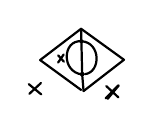
\begin{tikzpicture}[x=1em,y=1em,line cap=round,line join=round]
\draw[thick] (1.48,.04)--(0,1.12)--(1.48,2.25)--(3.03,1.13)--(1.57,0);
\draw[thick] (1.62,.61) .. controls (2.20,.68) and (2.20,1.76) .. (1.49,1.80) .. controls (.80,1.85) and (.76,.68) .. (1.52,.60);
\draw[thick] (1.48,2.25)--(1.52,.59)--(1.57,0);
\fill (1.49,1.80) circle (.074) (1.52,.61) circle (.085);
% Small internal x, then two larger external X-shaped marks.
\draw[thick] (.65,1.03)--(.85,1.32) (.65,1.29)--(.86,1.06);
\draw[thick] (-.39,-.10)--(.03,.29) (-.41,.25)--(.04,-.12);
\draw[thick] (2.37,-.26)--(2.82,.20) (2.39,.18)--(2.83,-.23);
\draw[thick] (2.44,-.28)--(2.84,.20);
\end{tikzpicture}}
\margin{Mais on aura $\unsure{X'|x'}_{L}\parallel Y'_{L}\Longrightarrow \unsure{X'|x'}\mathrel{\tikz[x=.55em,y=.60em,line cap=round]{\draw (0,-.12)--(0,1) (.48,-.12)--(.48,1) (-.06,.30)--(.54,.47) (-.05,.51)--(.53,.65);}}Y'$,\\ C'est un \unsure{contre-exple|contre-exemple|contre exemple} à l' : At $\parallel$, et a fortiori à \unsure{\deleted{ex}|ex} At 11 (cf GF $\underline{\overline{\mathrm{VI}}}$, p. 67,68)}%

% The thin vertical rule belongs beside the live axiom, not inside the title
% Critere. Ancien is an oblique interlinear word above/right of Soient;
% its verbal attachment remains uncertain although its letters are resolved.
\margin{\tikz[x=.5em,y=.5em]{\draw (0,0)--(0,4.25);}}%
\uline{At DD} 1 \tikz[baseline=(so.base)]{\node[inner sep=0pt] (so) {Soient};\node[anchor=south west,rotate=43,inner sep=0pt] at (so.north east) {\inserted{ancien}};} $X,Y\ \mathrel{\tikz[baseline=-.3ex,x=.48em,y=.65em,line cap=round]{\draw (.4,.9)..controls(-.05,.8)and(-.08,.04)..(.35,.04)..controls(.66,.04)and(.6,.6)..(.3,.63);\draw (.43,.33)--(.66,.35) (.33,.03)--(.36,-.1);}}\ X',Y'\in M$, $X\mathrel{\tikz[baseline=-.4ex,x=.65em,y=.65em]{\draw (0,1.1)--(1,.5)--(0,-.1) (1,1.1)--(0,.5)--(1,-.1);}}Y,\ X'\ll X,Y'\ll Y$. Posons $K=X\cap Y=\underset{Z\in\widetilde X\cap\widetilde Y}{\mathrm{Sup}}\,Z$. Alors $X'_{L}\mathrel{\tikz[baseline=-.4ex,x=.65em,y=.65em]{\draw (0,1.1)--(1,.5)--(0,-.1) (1,1.1)--(0,.5)--(1,-.1);}}Y'_{L}$ implique $X'\mathrel{\tikz[baseline=-.4ex,x=.65em,y=.65em]{\draw (0,1.1)--(1,.5)--(0,-.1) (1,1.1)--(0,.5)--(1,-.1);}}Y'$ \quad (NB \unsure{l'inverse|l'énoncé}\unsure{\, :|\, .|\,} \deleted{\unsure{est}} est tjrs vrai)
\normalmarginpar

\uline{Corollaire} 1 \quad \unsure{la|le} ``propriété'' ci dessus

\[
F\parallel G,\ F'\ll F,\ C'\ll G\ \Longrightarrow\ F'\parallel G'
\tag*{\makebox[0pt][r]{\makebox[\displaywidth][l]{\uline{Corollaire} 2}}}
\]

Plus gén. \quad Si $F\mathrel{\tikz[baseline=-.4ex,x=.65em,y=.65em]{\draw (0,1.1)--(1,.5)--(0,-.1) (1,1.1)--(0,.5)--(1,-.1);}}G,\ F'\ll F,\ C'\ll G$, alors
\[
 F'\parallel G'\ \Longleftrightarrow\ F'_{L}\parallel G'_{L}
\]
